% Created by tikzDevice version 0.9 on 2015-12-18 11:00:24
% !TEX encoding = UTF-8 Unicode
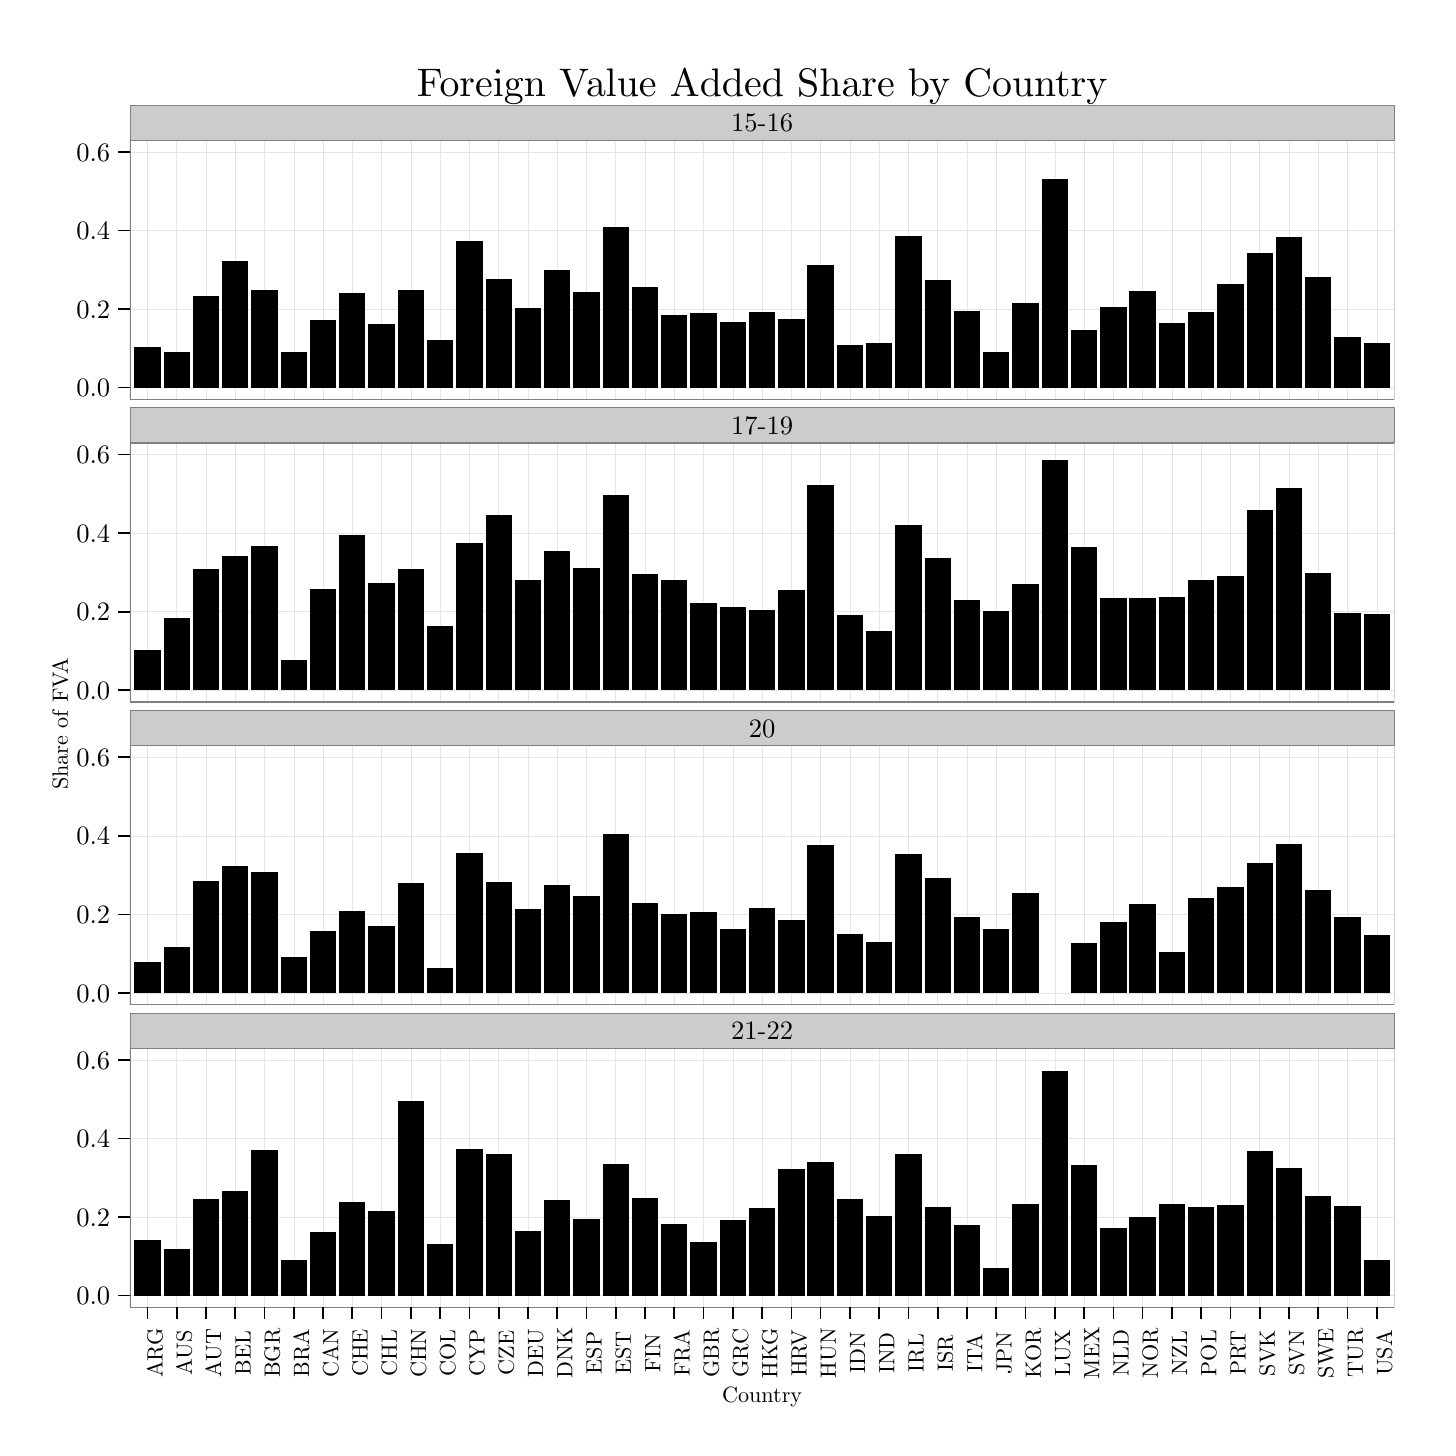
\begin{tikzpicture}[x=1pt,y=1pt]
\definecolor{fillColor}{RGB}{255,255,255}
\path[use as bounding box,fill=fillColor,fill opacity=0.00] (0,0) rectangle (505.89,505.89);
\begin{scope}
\path[clip] (  0.00,  0.00) rectangle (505.89,505.89);
\definecolor{drawColor}{RGB}{255,255,255}
\definecolor{fillColor}{RGB}{255,255,255}

\path[draw=drawColor,line width= 0.6pt,line join=round,line cap=round,fill=fillColor] (  0.00,  0.00) rectangle (505.89,505.89);
\end{scope}
\begin{scope}
\path[clip] ( 36.93,371.55) rectangle (493.85,465.27);
\definecolor{fillColor}{RGB}{255,255,255}

\path[fill=fillColor] ( 36.93,371.55) rectangle (493.85,465.27);
\definecolor{drawColor}{gray}{0.90}

\path[draw=drawColor,line width= 0.2pt,line join=round] ( 36.93,375.81) --
	(493.85,375.81);

\path[draw=drawColor,line width= 0.2pt,line join=round] ( 36.93,404.21) --
	(493.85,404.21);

\path[draw=drawColor,line width= 0.2pt,line join=round] ( 36.93,432.61) --
	(493.85,432.61);

\path[draw=drawColor,line width= 0.2pt,line join=round] ( 36.93,461.01) --
	(493.85,461.01);

\path[draw=drawColor,line width= 0.2pt,line join=round] ( 43.28,371.55) --
	( 43.28,465.27);

\path[draw=drawColor,line width= 0.2pt,line join=round] ( 53.85,371.55) --
	( 53.85,465.27);

\path[draw=drawColor,line width= 0.2pt,line join=round] ( 64.43,371.55) --
	( 64.43,465.27);

\path[draw=drawColor,line width= 0.2pt,line join=round] ( 75.01,371.55) --
	( 75.01,465.27);

\path[draw=drawColor,line width= 0.2pt,line join=round] ( 85.58,371.55) --
	( 85.58,465.27);

\path[draw=drawColor,line width= 0.2pt,line join=round] ( 96.16,371.55) --
	( 96.16,465.27);

\path[draw=drawColor,line width= 0.2pt,line join=round] (106.74,371.55) --
	(106.74,465.27);

\path[draw=drawColor,line width= 0.2pt,line join=round] (117.31,371.55) --
	(117.31,465.27);

\path[draw=drawColor,line width= 0.2pt,line join=round] (127.89,371.55) --
	(127.89,465.27);

\path[draw=drawColor,line width= 0.2pt,line join=round] (138.47,371.55) --
	(138.47,465.27);

\path[draw=drawColor,line width= 0.2pt,line join=round] (149.04,371.55) --
	(149.04,465.27);

\path[draw=drawColor,line width= 0.2pt,line join=round] (159.62,371.55) --
	(159.62,465.27);

\path[draw=drawColor,line width= 0.2pt,line join=round] (170.20,371.55) --
	(170.20,465.27);

\path[draw=drawColor,line width= 0.2pt,line join=round] (180.77,371.55) --
	(180.77,465.27);

\path[draw=drawColor,line width= 0.2pt,line join=round] (191.35,371.55) --
	(191.35,465.27);

\path[draw=drawColor,line width= 0.2pt,line join=round] (201.93,371.55) --
	(201.93,465.27);

\path[draw=drawColor,line width= 0.2pt,line join=round] (212.50,371.55) --
	(212.50,465.27);

\path[draw=drawColor,line width= 0.2pt,line join=round] (223.08,371.55) --
	(223.08,465.27);

\path[draw=drawColor,line width= 0.2pt,line join=round] (233.66,371.55) --
	(233.66,465.27);

\path[draw=drawColor,line width= 0.2pt,line join=round] (244.23,371.55) --
	(244.23,465.27);

\path[draw=drawColor,line width= 0.2pt,line join=round] (254.81,371.55) --
	(254.81,465.27);

\path[draw=drawColor,line width= 0.2pt,line join=round] (265.39,371.55) --
	(265.39,465.27);

\path[draw=drawColor,line width= 0.2pt,line join=round] (275.97,371.55) --
	(275.97,465.27);

\path[draw=drawColor,line width= 0.2pt,line join=round] (286.54,371.55) --
	(286.54,465.27);

\path[draw=drawColor,line width= 0.2pt,line join=round] (297.12,371.55) --
	(297.12,465.27);

\path[draw=drawColor,line width= 0.2pt,line join=round] (307.70,371.55) --
	(307.70,465.27);

\path[draw=drawColor,line width= 0.2pt,line join=round] (318.27,371.55) --
	(318.27,465.27);

\path[draw=drawColor,line width= 0.2pt,line join=round] (328.85,371.55) --
	(328.85,465.27);

\path[draw=drawColor,line width= 0.2pt,line join=round] (339.43,371.55) --
	(339.43,465.27);

\path[draw=drawColor,line width= 0.2pt,line join=round] (350.00,371.55) --
	(350.00,465.27);

\path[draw=drawColor,line width= 0.2pt,line join=round] (360.58,371.55) --
	(360.58,465.27);

\path[draw=drawColor,line width= 0.2pt,line join=round] (371.16,371.55) --
	(371.16,465.27);

\path[draw=drawColor,line width= 0.2pt,line join=round] (381.73,371.55) --
	(381.73,465.27);

\path[draw=drawColor,line width= 0.2pt,line join=round] (392.31,371.55) --
	(392.31,465.27);

\path[draw=drawColor,line width= 0.2pt,line join=round] (402.89,371.55) --
	(402.89,465.27);

\path[draw=drawColor,line width= 0.2pt,line join=round] (413.46,371.55) --
	(413.46,465.27);

\path[draw=drawColor,line width= 0.2pt,line join=round] (424.04,371.55) --
	(424.04,465.27);

\path[draw=drawColor,line width= 0.2pt,line join=round] (434.62,371.55) --
	(434.62,465.27);

\path[draw=drawColor,line width= 0.2pt,line join=round] (445.19,371.55) --
	(445.19,465.27);

\path[draw=drawColor,line width= 0.2pt,line join=round] (455.77,371.55) --
	(455.77,465.27);

\path[draw=drawColor,line width= 0.2pt,line join=round] (466.35,371.55) --
	(466.35,465.27);

\path[draw=drawColor,line width= 0.2pt,line join=round] (476.92,371.55) --
	(476.92,465.27);

\path[draw=drawColor,line width= 0.2pt,line join=round] (487.50,371.55) --
	(487.50,465.27);
\definecolor{fillColor}{RGB}{0,0,0}

\path[fill=fillColor] ( 38.52,375.81) rectangle ( 48.04,390.41);

\path[fill=fillColor] ( 49.09,375.81) rectangle ( 58.61,388.61);

\path[fill=fillColor] ( 59.67,375.81) rectangle ( 69.19,409.08);

\path[fill=fillColor] ( 70.25,375.81) rectangle ( 79.77,421.73);

\path[fill=fillColor] ( 80.83,375.81) rectangle ( 90.34,411.00);

\path[fill=fillColor] ( 91.40,375.81) rectangle (100.92,388.54);

\path[fill=fillColor] (101.98,375.81) rectangle (111.50,400.19);

\path[fill=fillColor] (112.56,375.81) rectangle (122.07,409.86);

\path[fill=fillColor] (123.13,375.81) rectangle (132.65,398.74);

\path[fill=fillColor] (133.71,375.81) rectangle (143.23,411.04);

\path[fill=fillColor] (144.29,375.81) rectangle (153.80,392.91);

\path[fill=fillColor] (154.86,375.81) rectangle (164.38,428.66);

\path[fill=fillColor] (165.44,375.81) rectangle (174.96,415.12);

\path[fill=fillColor] (176.02,375.81) rectangle (185.53,404.66);

\path[fill=fillColor] (186.59,375.81) rectangle (196.11,418.14);

\path[fill=fillColor] (197.17,375.81) rectangle (206.69,410.33);

\path[fill=fillColor] (207.75,375.81) rectangle (217.26,433.78);

\path[fill=fillColor] (218.32,375.81) rectangle (227.84,412.02);

\path[fill=fillColor] (228.90,375.81) rectangle (238.42,402.11);

\path[fill=fillColor] (239.48,375.81) rectangle (248.99,402.79);

\path[fill=fillColor] (250.05,375.81) rectangle (259.57,399.53);

\path[fill=fillColor] (260.63,375.81) rectangle (270.15,403.09);

\path[fill=fillColor] (271.21,375.81) rectangle (280.72,400.71);

\path[fill=fillColor] (281.78,375.81) rectangle (291.30,420.25);

\path[fill=fillColor] (292.36,375.81) rectangle (301.88,391.09);

\path[fill=fillColor] (302.94,375.81) rectangle (312.45,392.05);

\path[fill=fillColor] (313.51,375.81) rectangle (323.03,430.53);

\path[fill=fillColor] (324.09,375.81) rectangle (333.61,414.58);

\path[fill=fillColor] (334.67,375.81) rectangle (344.18,403.33);

\path[fill=fillColor] (345.24,375.81) rectangle (354.76,388.69);

\path[fill=fillColor] (355.82,375.81) rectangle (365.34,406.46);

\path[fill=fillColor] (366.40,375.81) rectangle (375.91,451.06);

\path[fill=fillColor] (376.97,375.81) rectangle (386.49,396.79);

\path[fill=fillColor] (387.55,375.81) rectangle (397.07,404.89);

\path[fill=fillColor] (398.13,375.81) rectangle (407.64,410.70);

\path[fill=fillColor] (408.70,375.81) rectangle (418.22,399.22);

\path[fill=fillColor] (419.28,375.81) rectangle (428.80,403.29);

\path[fill=fillColor] (429.86,375.81) rectangle (439.38,413.27);

\path[fill=fillColor] (440.43,375.81) rectangle (449.95,424.34);

\path[fill=fillColor] (451.01,375.81) rectangle (460.53,430.23);

\path[fill=fillColor] (461.59,375.81) rectangle (471.11,415.62);

\path[fill=fillColor] (472.16,375.81) rectangle (481.68,394.21);

\path[fill=fillColor] (482.74,375.81) rectangle (492.26,392.10);
\definecolor{drawColor}{gray}{0.50}

\path[draw=drawColor,line width= 0.6pt,line join=round,line cap=round] ( 36.93,371.55) rectangle (493.85,465.27);
\end{scope}
\begin{scope}
\path[clip] ( 36.93,262.18) rectangle (493.85,355.90);
\definecolor{fillColor}{RGB}{255,255,255}

\path[fill=fillColor] ( 36.93,262.18) rectangle (493.85,355.90);
\definecolor{drawColor}{gray}{0.90}

\path[draw=drawColor,line width= 0.2pt,line join=round] ( 36.93,266.44) --
	(493.85,266.44);

\path[draw=drawColor,line width= 0.2pt,line join=round] ( 36.93,294.84) --
	(493.85,294.84);

\path[draw=drawColor,line width= 0.2pt,line join=round] ( 36.93,323.24) --
	(493.85,323.24);

\path[draw=drawColor,line width= 0.2pt,line join=round] ( 36.93,351.64) --
	(493.85,351.64);

\path[draw=drawColor,line width= 0.2pt,line join=round] ( 43.28,262.18) --
	( 43.28,355.90);

\path[draw=drawColor,line width= 0.2pt,line join=round] ( 53.85,262.18) --
	( 53.85,355.90);

\path[draw=drawColor,line width= 0.2pt,line join=round] ( 64.43,262.18) --
	( 64.43,355.90);

\path[draw=drawColor,line width= 0.2pt,line join=round] ( 75.01,262.18) --
	( 75.01,355.90);

\path[draw=drawColor,line width= 0.2pt,line join=round] ( 85.58,262.18) --
	( 85.58,355.90);

\path[draw=drawColor,line width= 0.2pt,line join=round] ( 96.16,262.18) --
	( 96.16,355.90);

\path[draw=drawColor,line width= 0.2pt,line join=round] (106.74,262.18) --
	(106.74,355.90);

\path[draw=drawColor,line width= 0.2pt,line join=round] (117.31,262.18) --
	(117.31,355.90);

\path[draw=drawColor,line width= 0.2pt,line join=round] (127.89,262.18) --
	(127.89,355.90);

\path[draw=drawColor,line width= 0.2pt,line join=round] (138.47,262.18) --
	(138.47,355.90);

\path[draw=drawColor,line width= 0.2pt,line join=round] (149.04,262.18) --
	(149.04,355.90);

\path[draw=drawColor,line width= 0.2pt,line join=round] (159.62,262.18) --
	(159.62,355.90);

\path[draw=drawColor,line width= 0.2pt,line join=round] (170.20,262.18) --
	(170.20,355.90);

\path[draw=drawColor,line width= 0.2pt,line join=round] (180.77,262.18) --
	(180.77,355.90);

\path[draw=drawColor,line width= 0.2pt,line join=round] (191.35,262.18) --
	(191.35,355.90);

\path[draw=drawColor,line width= 0.2pt,line join=round] (201.93,262.18) --
	(201.93,355.90);

\path[draw=drawColor,line width= 0.2pt,line join=round] (212.50,262.18) --
	(212.50,355.90);

\path[draw=drawColor,line width= 0.2pt,line join=round] (223.08,262.18) --
	(223.08,355.90);

\path[draw=drawColor,line width= 0.2pt,line join=round] (233.66,262.18) --
	(233.66,355.90);

\path[draw=drawColor,line width= 0.2pt,line join=round] (244.23,262.18) --
	(244.23,355.90);

\path[draw=drawColor,line width= 0.2pt,line join=round] (254.81,262.18) --
	(254.81,355.90);

\path[draw=drawColor,line width= 0.2pt,line join=round] (265.39,262.18) --
	(265.39,355.90);

\path[draw=drawColor,line width= 0.2pt,line join=round] (275.97,262.18) --
	(275.97,355.90);

\path[draw=drawColor,line width= 0.2pt,line join=round] (286.54,262.18) --
	(286.54,355.90);

\path[draw=drawColor,line width= 0.2pt,line join=round] (297.12,262.18) --
	(297.12,355.90);

\path[draw=drawColor,line width= 0.2pt,line join=round] (307.70,262.18) --
	(307.70,355.90);

\path[draw=drawColor,line width= 0.2pt,line join=round] (318.27,262.18) --
	(318.27,355.90);

\path[draw=drawColor,line width= 0.2pt,line join=round] (328.85,262.18) --
	(328.85,355.90);

\path[draw=drawColor,line width= 0.2pt,line join=round] (339.43,262.18) --
	(339.43,355.90);

\path[draw=drawColor,line width= 0.2pt,line join=round] (350.00,262.18) --
	(350.00,355.90);

\path[draw=drawColor,line width= 0.2pt,line join=round] (360.58,262.18) --
	(360.58,355.90);

\path[draw=drawColor,line width= 0.2pt,line join=round] (371.16,262.18) --
	(371.16,355.90);

\path[draw=drawColor,line width= 0.2pt,line join=round] (381.73,262.18) --
	(381.73,355.90);

\path[draw=drawColor,line width= 0.2pt,line join=round] (392.31,262.18) --
	(392.31,355.90);

\path[draw=drawColor,line width= 0.2pt,line join=round] (402.89,262.18) --
	(402.89,355.90);

\path[draw=drawColor,line width= 0.2pt,line join=round] (413.46,262.18) --
	(413.46,355.90);

\path[draw=drawColor,line width= 0.2pt,line join=round] (424.04,262.18) --
	(424.04,355.90);

\path[draw=drawColor,line width= 0.2pt,line join=round] (434.62,262.18) --
	(434.62,355.90);

\path[draw=drawColor,line width= 0.2pt,line join=round] (445.19,262.18) --
	(445.19,355.90);

\path[draw=drawColor,line width= 0.2pt,line join=round] (455.77,262.18) --
	(455.77,355.90);

\path[draw=drawColor,line width= 0.2pt,line join=round] (466.35,262.18) --
	(466.35,355.90);

\path[draw=drawColor,line width= 0.2pt,line join=round] (476.92,262.18) --
	(476.92,355.90);

\path[draw=drawColor,line width= 0.2pt,line join=round] (487.50,262.18) --
	(487.50,355.90);
\definecolor{fillColor}{RGB}{0,0,0}

\path[fill=fillColor] ( 38.52,266.44) rectangle ( 48.04,280.99);

\path[fill=fillColor] ( 49.09,266.44) rectangle ( 58.61,292.69);

\path[fill=fillColor] ( 59.67,266.44) rectangle ( 69.19,310.40);

\path[fill=fillColor] ( 70.25,266.44) rectangle ( 79.77,314.99);

\path[fill=fillColor] ( 80.83,266.44) rectangle ( 90.34,318.49);

\path[fill=fillColor] ( 91.40,266.44) rectangle (100.92,277.50);

\path[fill=fillColor] (101.98,266.44) rectangle (111.50,303.21);

\path[fill=fillColor] (112.56,266.44) rectangle (122.07,322.59);

\path[fill=fillColor] (123.13,266.44) rectangle (132.65,305.13);

\path[fill=fillColor] (133.71,266.44) rectangle (143.23,310.40);

\path[fill=fillColor] (144.29,266.44) rectangle (153.80,289.53);

\path[fill=fillColor] (154.86,266.44) rectangle (164.38,319.60);

\path[fill=fillColor] (165.44,266.44) rectangle (174.96,329.88);

\path[fill=fillColor] (176.02,266.44) rectangle (185.53,306.36);

\path[fill=fillColor] (186.59,266.44) rectangle (196.11,316.96);

\path[fill=fillColor] (197.17,266.44) rectangle (206.69,310.58);

\path[fill=fillColor] (207.75,266.44) rectangle (217.26,336.88);

\path[fill=fillColor] (218.32,266.44) rectangle (227.84,308.43);

\path[fill=fillColor] (228.90,266.44) rectangle (238.42,306.27);

\path[fill=fillColor] (239.48,266.44) rectangle (248.99,298.11);

\path[fill=fillColor] (250.05,266.44) rectangle (259.57,296.47);

\path[fill=fillColor] (260.63,266.44) rectangle (270.15,295.51);

\path[fill=fillColor] (271.21,266.44) rectangle (280.72,302.58);

\path[fill=fillColor] (281.78,266.44) rectangle (291.30,340.81);

\path[fill=fillColor] (292.36,266.44) rectangle (301.88,293.81);

\path[fill=fillColor] (302.94,266.44) rectangle (312.45,287.71);

\path[fill=fillColor] (313.51,266.44) rectangle (323.03,326.04);

\path[fill=fillColor] (324.09,266.44) rectangle (333.61,314.30);

\path[fill=fillColor] (334.67,266.44) rectangle (344.18,299.01);

\path[fill=fillColor] (345.24,266.44) rectangle (354.76,295.11);

\path[fill=fillColor] (355.82,266.44) rectangle (365.34,304.88);

\path[fill=fillColor] (366.40,266.44) rectangle (375.91,349.50);

\path[fill=fillColor] (376.97,266.44) rectangle (386.49,318.13);

\path[fill=fillColor] (387.55,266.44) rectangle (397.07,299.74);

\path[fill=fillColor] (398.13,266.44) rectangle (407.64,299.81);

\path[fill=fillColor] (408.70,266.44) rectangle (418.22,300.18);

\path[fill=fillColor] (419.28,266.44) rectangle (428.80,306.28);

\path[fill=fillColor] (429.86,266.44) rectangle (439.38,307.91);

\path[fill=fillColor] (440.43,266.44) rectangle (449.95,331.42);

\path[fill=fillColor] (451.01,266.44) rectangle (460.53,339.43);

\path[fill=fillColor] (461.59,266.44) rectangle (471.11,308.97);

\path[fill=fillColor] (472.16,266.44) rectangle (481.68,294.22);

\path[fill=fillColor] (482.74,266.44) rectangle (492.26,294.09);
\definecolor{drawColor}{gray}{0.50}

\path[draw=drawColor,line width= 0.6pt,line join=round,line cap=round] ( 36.93,262.18) rectangle (493.85,355.90);
\end{scope}
\begin{scope}
\path[clip] ( 36.93,152.81) rectangle (493.85,246.53);
\definecolor{fillColor}{RGB}{255,255,255}

\path[fill=fillColor] ( 36.93,152.81) rectangle (493.85,246.53);
\definecolor{drawColor}{gray}{0.90}

\path[draw=drawColor,line width= 0.2pt,line join=round] ( 36.93,157.07) --
	(493.85,157.07);

\path[draw=drawColor,line width= 0.2pt,line join=round] ( 36.93,185.47) --
	(493.85,185.47);

\path[draw=drawColor,line width= 0.2pt,line join=round] ( 36.93,213.87) --
	(493.85,213.87);

\path[draw=drawColor,line width= 0.2pt,line join=round] ( 36.93,242.27) --
	(493.85,242.27);

\path[draw=drawColor,line width= 0.2pt,line join=round] ( 43.28,152.81) --
	( 43.28,246.53);

\path[draw=drawColor,line width= 0.2pt,line join=round] ( 53.85,152.81) --
	( 53.85,246.53);

\path[draw=drawColor,line width= 0.2pt,line join=round] ( 64.43,152.81) --
	( 64.43,246.53);

\path[draw=drawColor,line width= 0.2pt,line join=round] ( 75.01,152.81) --
	( 75.01,246.53);

\path[draw=drawColor,line width= 0.2pt,line join=round] ( 85.58,152.81) --
	( 85.58,246.53);

\path[draw=drawColor,line width= 0.2pt,line join=round] ( 96.16,152.81) --
	( 96.16,246.53);

\path[draw=drawColor,line width= 0.2pt,line join=round] (106.74,152.81) --
	(106.74,246.53);

\path[draw=drawColor,line width= 0.2pt,line join=round] (117.31,152.81) --
	(117.31,246.53);

\path[draw=drawColor,line width= 0.2pt,line join=round] (127.89,152.81) --
	(127.89,246.53);

\path[draw=drawColor,line width= 0.2pt,line join=round] (138.47,152.81) --
	(138.47,246.53);

\path[draw=drawColor,line width= 0.2pt,line join=round] (149.04,152.81) --
	(149.04,246.53);

\path[draw=drawColor,line width= 0.2pt,line join=round] (159.62,152.81) --
	(159.62,246.53);

\path[draw=drawColor,line width= 0.2pt,line join=round] (170.20,152.81) --
	(170.20,246.53);

\path[draw=drawColor,line width= 0.2pt,line join=round] (180.77,152.81) --
	(180.77,246.53);

\path[draw=drawColor,line width= 0.2pt,line join=round] (191.35,152.81) --
	(191.35,246.53);

\path[draw=drawColor,line width= 0.2pt,line join=round] (201.93,152.81) --
	(201.93,246.53);

\path[draw=drawColor,line width= 0.2pt,line join=round] (212.50,152.81) --
	(212.50,246.53);

\path[draw=drawColor,line width= 0.2pt,line join=round] (223.08,152.81) --
	(223.08,246.53);

\path[draw=drawColor,line width= 0.2pt,line join=round] (233.66,152.81) --
	(233.66,246.53);

\path[draw=drawColor,line width= 0.2pt,line join=round] (244.23,152.81) --
	(244.23,246.53);

\path[draw=drawColor,line width= 0.2pt,line join=round] (254.81,152.81) --
	(254.81,246.53);

\path[draw=drawColor,line width= 0.2pt,line join=round] (265.39,152.81) --
	(265.39,246.53);

\path[draw=drawColor,line width= 0.2pt,line join=round] (275.97,152.81) --
	(275.97,246.53);

\path[draw=drawColor,line width= 0.2pt,line join=round] (286.54,152.81) --
	(286.54,246.53);

\path[draw=drawColor,line width= 0.2pt,line join=round] (297.12,152.81) --
	(297.12,246.53);

\path[draw=drawColor,line width= 0.2pt,line join=round] (307.70,152.81) --
	(307.70,246.53);

\path[draw=drawColor,line width= 0.2pt,line join=round] (318.27,152.81) --
	(318.27,246.53);

\path[draw=drawColor,line width= 0.2pt,line join=round] (328.85,152.81) --
	(328.85,246.53);

\path[draw=drawColor,line width= 0.2pt,line join=round] (339.43,152.81) --
	(339.43,246.53);

\path[draw=drawColor,line width= 0.2pt,line join=round] (350.00,152.81) --
	(350.00,246.53);

\path[draw=drawColor,line width= 0.2pt,line join=round] (360.58,152.81) --
	(360.58,246.53);

\path[draw=drawColor,line width= 0.2pt,line join=round] (371.16,152.81) --
	(371.16,246.53);

\path[draw=drawColor,line width= 0.2pt,line join=round] (381.73,152.81) --
	(381.73,246.53);

\path[draw=drawColor,line width= 0.2pt,line join=round] (392.31,152.81) --
	(392.31,246.53);

\path[draw=drawColor,line width= 0.2pt,line join=round] (402.89,152.81) --
	(402.89,246.53);

\path[draw=drawColor,line width= 0.2pt,line join=round] (413.46,152.81) --
	(413.46,246.53);

\path[draw=drawColor,line width= 0.2pt,line join=round] (424.04,152.81) --
	(424.04,246.53);

\path[draw=drawColor,line width= 0.2pt,line join=round] (434.62,152.81) --
	(434.62,246.53);

\path[draw=drawColor,line width= 0.2pt,line join=round] (445.19,152.81) --
	(445.19,246.53);

\path[draw=drawColor,line width= 0.2pt,line join=round] (455.77,152.81) --
	(455.77,246.53);

\path[draw=drawColor,line width= 0.2pt,line join=round] (466.35,152.81) --
	(466.35,246.53);

\path[draw=drawColor,line width= 0.2pt,line join=round] (476.92,152.81) --
	(476.92,246.53);

\path[draw=drawColor,line width= 0.2pt,line join=round] (487.50,152.81) --
	(487.50,246.53);
\definecolor{fillColor}{RGB}{0,0,0}

\path[fill=fillColor] ( 38.52,157.07) rectangle ( 48.04,168.14);

\path[fill=fillColor] ( 49.09,157.07) rectangle ( 58.61,173.72);

\path[fill=fillColor] ( 59.67,157.07) rectangle ( 69.19,197.49);

\path[fill=fillColor] ( 70.25,157.07) rectangle ( 79.77,202.80);

\path[fill=fillColor] ( 80.83,157.07) rectangle ( 90.34,200.96);

\path[fill=fillColor] ( 91.40,157.07) rectangle (100.92,170.16);

\path[fill=fillColor] (101.98,157.07) rectangle (111.50,179.30);

\path[fill=fillColor] (112.56,157.07) rectangle (122.07,186.55);

\path[fill=fillColor] (123.13,157.07) rectangle (132.65,181.13);

\path[fill=fillColor] (133.71,157.07) rectangle (143.23,196.78);

\path[fill=fillColor] (144.29,157.07) rectangle (153.80,166.12);

\path[fill=fillColor] (154.86,157.07) rectangle (164.38,207.77);

\path[fill=fillColor] (165.44,157.07) rectangle (174.96,197.22);

\path[fill=fillColor] (176.02,157.07) rectangle (185.53,187.38);

\path[fill=fillColor] (186.59,157.07) rectangle (196.11,196.15);

\path[fill=fillColor] (197.17,157.07) rectangle (206.69,192.17);

\path[fill=fillColor] (207.75,157.07) rectangle (217.26,214.65);

\path[fill=fillColor] (218.32,157.07) rectangle (227.84,189.69);

\path[fill=fillColor] (228.90,157.07) rectangle (238.42,185.67);

\path[fill=fillColor] (239.48,157.07) rectangle (248.99,186.51);

\path[fill=fillColor] (250.05,157.07) rectangle (259.57,180.20);

\path[fill=fillColor] (260.63,157.07) rectangle (270.15,187.76);

\path[fill=fillColor] (271.21,157.07) rectangle (280.72,183.35);

\path[fill=fillColor] (281.78,157.07) rectangle (291.30,210.66);

\path[fill=fillColor] (292.36,157.07) rectangle (301.88,178.22);

\path[fill=fillColor] (302.94,157.07) rectangle (312.45,175.51);

\path[fill=fillColor] (313.51,157.07) rectangle (323.03,207.19);

\path[fill=fillColor] (324.09,157.07) rectangle (333.61,198.76);

\path[fill=fillColor] (334.67,157.07) rectangle (344.18,184.70);

\path[fill=fillColor] (345.24,157.07) rectangle (354.76,180.02);

\path[fill=fillColor] (355.82,157.07) rectangle (365.34,193.06);

\path[fill=fillColor] (376.97,157.07) rectangle (386.49,175.06);

\path[fill=fillColor] (387.55,157.07) rectangle (397.07,182.74);

\path[fill=fillColor] (398.13,157.07) rectangle (407.64,189.30);

\path[fill=fillColor] (408.70,157.07) rectangle (418.22,171.76);

\path[fill=fillColor] (419.28,157.07) rectangle (428.80,191.50);

\path[fill=fillColor] (429.86,157.07) rectangle (439.38,195.48);

\path[fill=fillColor] (440.43,157.07) rectangle (449.95,204.20);

\path[fill=fillColor] (451.01,157.07) rectangle (460.53,210.74);

\path[fill=fillColor] (461.59,157.07) rectangle (471.11,194.43);

\path[fill=fillColor] (472.16,157.07) rectangle (481.68,184.47);

\path[fill=fillColor] (482.74,157.07) rectangle (492.26,178.04);
\definecolor{drawColor}{gray}{0.50}

\path[draw=drawColor,line width= 0.6pt,line join=round,line cap=round] ( 36.93,152.81) rectangle (493.85,246.53);
\end{scope}
\begin{scope}
\path[clip] ( 36.93, 43.44) rectangle (493.85,137.16);
\definecolor{fillColor}{RGB}{255,255,255}

\path[fill=fillColor] ( 36.93, 43.44) rectangle (493.85,137.16);
\definecolor{drawColor}{gray}{0.90}

\path[draw=drawColor,line width= 0.2pt,line join=round] ( 36.93, 47.70) --
	(493.85, 47.70);

\path[draw=drawColor,line width= 0.2pt,line join=round] ( 36.93, 76.10) --
	(493.85, 76.10);

\path[draw=drawColor,line width= 0.2pt,line join=round] ( 36.93,104.50) --
	(493.85,104.50);

\path[draw=drawColor,line width= 0.2pt,line join=round] ( 36.93,132.90) --
	(493.85,132.90);

\path[draw=drawColor,line width= 0.2pt,line join=round] ( 43.28, 43.44) --
	( 43.28,137.16);

\path[draw=drawColor,line width= 0.2pt,line join=round] ( 53.85, 43.44) --
	( 53.85,137.16);

\path[draw=drawColor,line width= 0.2pt,line join=round] ( 64.43, 43.44) --
	( 64.43,137.16);

\path[draw=drawColor,line width= 0.2pt,line join=round] ( 75.01, 43.44) --
	( 75.01,137.16);

\path[draw=drawColor,line width= 0.2pt,line join=round] ( 85.58, 43.44) --
	( 85.58,137.16);

\path[draw=drawColor,line width= 0.2pt,line join=round] ( 96.16, 43.44) --
	( 96.16,137.16);

\path[draw=drawColor,line width= 0.2pt,line join=round] (106.74, 43.44) --
	(106.74,137.16);

\path[draw=drawColor,line width= 0.2pt,line join=round] (117.31, 43.44) --
	(117.31,137.16);

\path[draw=drawColor,line width= 0.2pt,line join=round] (127.89, 43.44) --
	(127.89,137.16);

\path[draw=drawColor,line width= 0.2pt,line join=round] (138.47, 43.44) --
	(138.47,137.16);

\path[draw=drawColor,line width= 0.2pt,line join=round] (149.04, 43.44) --
	(149.04,137.16);

\path[draw=drawColor,line width= 0.2pt,line join=round] (159.62, 43.44) --
	(159.62,137.16);

\path[draw=drawColor,line width= 0.2pt,line join=round] (170.20, 43.44) --
	(170.20,137.16);

\path[draw=drawColor,line width= 0.2pt,line join=round] (180.77, 43.44) --
	(180.77,137.16);

\path[draw=drawColor,line width= 0.2pt,line join=round] (191.35, 43.44) --
	(191.35,137.16);

\path[draw=drawColor,line width= 0.2pt,line join=round] (201.93, 43.44) --
	(201.93,137.16);

\path[draw=drawColor,line width= 0.2pt,line join=round] (212.50, 43.44) --
	(212.50,137.16);

\path[draw=drawColor,line width= 0.2pt,line join=round] (223.08, 43.44) --
	(223.08,137.16);

\path[draw=drawColor,line width= 0.2pt,line join=round] (233.66, 43.44) --
	(233.66,137.16);

\path[draw=drawColor,line width= 0.2pt,line join=round] (244.23, 43.44) --
	(244.23,137.16);

\path[draw=drawColor,line width= 0.2pt,line join=round] (254.81, 43.44) --
	(254.81,137.16);

\path[draw=drawColor,line width= 0.2pt,line join=round] (265.39, 43.44) --
	(265.39,137.16);

\path[draw=drawColor,line width= 0.2pt,line join=round] (275.97, 43.44) --
	(275.97,137.16);

\path[draw=drawColor,line width= 0.2pt,line join=round] (286.54, 43.44) --
	(286.54,137.16);

\path[draw=drawColor,line width= 0.2pt,line join=round] (297.12, 43.44) --
	(297.12,137.16);

\path[draw=drawColor,line width= 0.2pt,line join=round] (307.70, 43.44) --
	(307.70,137.16);

\path[draw=drawColor,line width= 0.2pt,line join=round] (318.27, 43.44) --
	(318.27,137.16);

\path[draw=drawColor,line width= 0.2pt,line join=round] (328.85, 43.44) --
	(328.85,137.16);

\path[draw=drawColor,line width= 0.2pt,line join=round] (339.43, 43.44) --
	(339.43,137.16);

\path[draw=drawColor,line width= 0.2pt,line join=round] (350.00, 43.44) --
	(350.00,137.16);

\path[draw=drawColor,line width= 0.2pt,line join=round] (360.58, 43.44) --
	(360.58,137.16);

\path[draw=drawColor,line width= 0.2pt,line join=round] (371.16, 43.44) --
	(371.16,137.16);

\path[draw=drawColor,line width= 0.2pt,line join=round] (381.73, 43.44) --
	(381.73,137.16);

\path[draw=drawColor,line width= 0.2pt,line join=round] (392.31, 43.44) --
	(392.31,137.16);

\path[draw=drawColor,line width= 0.2pt,line join=round] (402.89, 43.44) --
	(402.89,137.16);

\path[draw=drawColor,line width= 0.2pt,line join=round] (413.46, 43.44) --
	(413.46,137.16);

\path[draw=drawColor,line width= 0.2pt,line join=round] (424.04, 43.44) --
	(424.04,137.16);

\path[draw=drawColor,line width= 0.2pt,line join=round] (434.62, 43.44) --
	(434.62,137.16);

\path[draw=drawColor,line width= 0.2pt,line join=round] (445.19, 43.44) --
	(445.19,137.16);

\path[draw=drawColor,line width= 0.2pt,line join=round] (455.77, 43.44) --
	(455.77,137.16);

\path[draw=drawColor,line width= 0.2pt,line join=round] (466.35, 43.44) --
	(466.35,137.16);

\path[draw=drawColor,line width= 0.2pt,line join=round] (476.92, 43.44) --
	(476.92,137.16);

\path[draw=drawColor,line width= 0.2pt,line join=round] (487.50, 43.44) --
	(487.50,137.16);
\definecolor{fillColor}{RGB}{0,0,0}

\path[fill=fillColor] ( 38.52, 47.70) rectangle ( 48.04, 67.93);

\path[fill=fillColor] ( 49.09, 47.70) rectangle ( 58.61, 64.62);

\path[fill=fillColor] ( 59.67, 47.70) rectangle ( 69.19, 82.70);

\path[fill=fillColor] ( 70.25, 47.70) rectangle ( 79.77, 85.41);

\path[fill=fillColor] ( 80.83, 47.70) rectangle ( 90.34,100.23);

\path[fill=fillColor] ( 91.40, 47.70) rectangle (100.92, 60.45);

\path[fill=fillColor] (101.98, 47.70) rectangle (111.50, 70.68);

\path[fill=fillColor] (112.56, 47.70) rectangle (122.07, 81.55);

\path[fill=fillColor] (123.13, 47.70) rectangle (132.65, 78.13);

\path[fill=fillColor] (133.71, 47.70) rectangle (143.23,118.00);

\path[fill=fillColor] (144.29, 47.70) rectangle (153.80, 66.50);

\path[fill=fillColor] (154.86, 47.70) rectangle (164.38,100.74);

\path[fill=fillColor] (165.44, 47.70) rectangle (174.96, 98.94);

\path[fill=fillColor] (176.02, 47.70) rectangle (185.53, 71.21);

\path[fill=fillColor] (186.59, 47.70) rectangle (196.11, 82.27);

\path[fill=fillColor] (197.17, 47.70) rectangle (206.69, 75.30);

\path[fill=fillColor] (207.75, 47.70) rectangle (217.26, 95.42);

\path[fill=fillColor] (218.32, 47.70) rectangle (227.84, 83.14);

\path[fill=fillColor] (228.90, 47.70) rectangle (238.42, 73.60);

\path[fill=fillColor] (239.48, 47.70) rectangle (248.99, 67.14);

\path[fill=fillColor] (250.05, 47.70) rectangle (259.57, 75.22);

\path[fill=fillColor] (260.63, 47.70) rectangle (270.15, 79.21);

\path[fill=fillColor] (271.21, 47.70) rectangle (280.72, 93.29);

\path[fill=fillColor] (281.78, 47.70) rectangle (291.30, 95.94);

\path[fill=fillColor] (292.36, 47.70) rectangle (301.88, 82.55);

\path[fill=fillColor] (302.94, 47.70) rectangle (312.45, 76.46);

\path[fill=fillColor] (313.51, 47.70) rectangle (323.03, 99.05);

\path[fill=fillColor] (324.09, 47.70) rectangle (333.61, 79.82);

\path[fill=fillColor] (334.67, 47.70) rectangle (344.18, 73.27);

\path[fill=fillColor] (345.24, 47.70) rectangle (354.76, 57.77);

\path[fill=fillColor] (355.82, 47.70) rectangle (365.34, 80.68);

\path[fill=fillColor] (366.40, 47.70) rectangle (375.91,129.05);

\path[fill=fillColor] (376.97, 47.70) rectangle (386.49, 94.74);

\path[fill=fillColor] (387.55, 47.70) rectangle (397.07, 72.06);

\path[fill=fillColor] (398.13, 47.70) rectangle (407.64, 76.05);

\path[fill=fillColor] (408.70, 47.70) rectangle (418.22, 80.95);

\path[fill=fillColor] (419.28, 47.70) rectangle (428.80, 79.57);

\path[fill=fillColor] (429.86, 47.70) rectangle (439.38, 80.34);

\path[fill=fillColor] (440.43, 47.70) rectangle (449.95,100.07);

\path[fill=fillColor] (451.01, 47.70) rectangle (460.53, 93.87);

\path[fill=fillColor] (461.59, 47.70) rectangle (471.11, 83.56);

\path[fill=fillColor] (472.16, 47.70) rectangle (481.68, 80.16);

\path[fill=fillColor] (482.74, 47.70) rectangle (492.26, 60.48);
\definecolor{drawColor}{gray}{0.50}

\path[draw=drawColor,line width= 0.6pt,line join=round,line cap=round] ( 36.93, 43.44) rectangle (493.85,137.16);
\end{scope}
\begin{scope}
\path[clip] (  0.00,  0.00) rectangle (505.89,505.89);
\definecolor{drawColor}{gray}{0.50}
\definecolor{fillColor}{gray}{0.80}

\path[draw=drawColor,line width= 0.2pt,line join=round,line cap=round,fill=fillColor] ( 36.93,465.27) rectangle (493.85,477.90);
\definecolor{drawColor}{RGB}{0,0,0}

\node[text=drawColor,anchor=base,inner sep=0pt, outer sep=0pt, scale=  0.96] at (265.39,468.28) {15-16};
\end{scope}
\begin{scope}
\path[clip] (  0.00,  0.00) rectangle (505.89,505.89);
\definecolor{drawColor}{gray}{0.50}
\definecolor{fillColor}{gray}{0.80}

\path[draw=drawColor,line width= 0.2pt,line join=round,line cap=round,fill=fillColor] ( 36.93,355.90) rectangle (493.85,368.54);
\definecolor{drawColor}{RGB}{0,0,0}

\node[text=drawColor,anchor=base,inner sep=0pt, outer sep=0pt, scale=  0.96] at (265.39,358.91) {17-19};
\end{scope}
\begin{scope}
\path[clip] (  0.00,  0.00) rectangle (505.89,505.89);
\definecolor{drawColor}{gray}{0.50}
\definecolor{fillColor}{gray}{0.80}

\path[draw=drawColor,line width= 0.2pt,line join=round,line cap=round,fill=fillColor] ( 36.93,246.53) rectangle (493.85,259.17);
\definecolor{drawColor}{RGB}{0,0,0}

\node[text=drawColor,anchor=base,inner sep=0pt, outer sep=0pt, scale=  0.96] at (265.39,249.54) {20};
\end{scope}
\begin{scope}
\path[clip] (  0.00,  0.00) rectangle (505.89,505.89);
\definecolor{drawColor}{gray}{0.50}
\definecolor{fillColor}{gray}{0.80}

\path[draw=drawColor,line width= 0.2pt,line join=round,line cap=round,fill=fillColor] ( 36.93,137.16) rectangle (493.85,149.80);
\definecolor{drawColor}{RGB}{0,0,0}

\node[text=drawColor,anchor=base,inner sep=0pt, outer sep=0pt, scale=  0.96] at (265.39,140.18) {21-22};
\end{scope}
\begin{scope}
\path[clip] (  0.00,  0.00) rectangle (505.89,505.89);
\definecolor{drawColor}{RGB}{0,0,0}

\node[text=drawColor,anchor=base east,inner sep=0pt, outer sep=0pt, scale=  0.96] at ( 29.82,372.50) {0.0};

\node[text=drawColor,anchor=base east,inner sep=0pt, outer sep=0pt, scale=  0.96] at ( 29.82,400.90) {0.2};

\node[text=drawColor,anchor=base east,inner sep=0pt, outer sep=0pt, scale=  0.96] at ( 29.82,429.30) {0.4};

\node[text=drawColor,anchor=base east,inner sep=0pt, outer sep=0pt, scale=  0.96] at ( 29.82,457.70) {0.6};
\end{scope}
\begin{scope}
\path[clip] (  0.00,  0.00) rectangle (505.89,505.89);
\definecolor{drawColor}{RGB}{0,0,0}

\path[draw=drawColor,line width= 0.6pt,line join=round] ( 32.66,375.81) --
	( 36.93,375.81);

\path[draw=drawColor,line width= 0.6pt,line join=round] ( 32.66,404.21) --
	( 36.93,404.21);

\path[draw=drawColor,line width= 0.6pt,line join=round] ( 32.66,432.61) --
	( 36.93,432.61);

\path[draw=drawColor,line width= 0.6pt,line join=round] ( 32.66,461.01) --
	( 36.93,461.01);
\end{scope}
\begin{scope}
\path[clip] (  0.00,  0.00) rectangle (505.89,505.89);
\definecolor{drawColor}{RGB}{0,0,0}

\node[text=drawColor,anchor=base east,inner sep=0pt, outer sep=0pt, scale=  0.96] at ( 29.82,263.13) {0.0};

\node[text=drawColor,anchor=base east,inner sep=0pt, outer sep=0pt, scale=  0.96] at ( 29.82,291.53) {0.2};

\node[text=drawColor,anchor=base east,inner sep=0pt, outer sep=0pt, scale=  0.96] at ( 29.82,319.93) {0.4};

\node[text=drawColor,anchor=base east,inner sep=0pt, outer sep=0pt, scale=  0.96] at ( 29.82,348.34) {0.6};
\end{scope}
\begin{scope}
\path[clip] (  0.00,  0.00) rectangle (505.89,505.89);
\definecolor{drawColor}{RGB}{0,0,0}

\path[draw=drawColor,line width= 0.6pt,line join=round] ( 32.66,266.44) --
	( 36.93,266.44);

\path[draw=drawColor,line width= 0.6pt,line join=round] ( 32.66,294.84) --
	( 36.93,294.84);

\path[draw=drawColor,line width= 0.6pt,line join=round] ( 32.66,323.24) --
	( 36.93,323.24);

\path[draw=drawColor,line width= 0.6pt,line join=round] ( 32.66,351.64) --
	( 36.93,351.64);
\end{scope}
\begin{scope}
\path[clip] (  0.00,  0.00) rectangle (505.89,505.89);
\definecolor{drawColor}{RGB}{0,0,0}

\node[text=drawColor,anchor=base east,inner sep=0pt, outer sep=0pt, scale=  0.96] at ( 29.82,153.76) {0.0};

\node[text=drawColor,anchor=base east,inner sep=0pt, outer sep=0pt, scale=  0.96] at ( 29.82,182.17) {0.2};

\node[text=drawColor,anchor=base east,inner sep=0pt, outer sep=0pt, scale=  0.96] at ( 29.82,210.57) {0.4};

\node[text=drawColor,anchor=base east,inner sep=0pt, outer sep=0pt, scale=  0.96] at ( 29.82,238.97) {0.6};
\end{scope}
\begin{scope}
\path[clip] (  0.00,  0.00) rectangle (505.89,505.89);
\definecolor{drawColor}{RGB}{0,0,0}

\path[draw=drawColor,line width= 0.6pt,line join=round] ( 32.66,157.07) --
	( 36.93,157.07);

\path[draw=drawColor,line width= 0.6pt,line join=round] ( 32.66,185.47) --
	( 36.93,185.47);

\path[draw=drawColor,line width= 0.6pt,line join=round] ( 32.66,213.87) --
	( 36.93,213.87);

\path[draw=drawColor,line width= 0.6pt,line join=round] ( 32.66,242.27) --
	( 36.93,242.27);
\end{scope}
\begin{scope}
\path[clip] (  0.00,  0.00) rectangle (505.89,505.89);
\definecolor{drawColor}{RGB}{0,0,0}

\node[text=drawColor,anchor=base east,inner sep=0pt, outer sep=0pt, scale=  0.96] at ( 29.82, 44.40) {0.0};

\node[text=drawColor,anchor=base east,inner sep=0pt, outer sep=0pt, scale=  0.96] at ( 29.82, 72.80) {0.2};

\node[text=drawColor,anchor=base east,inner sep=0pt, outer sep=0pt, scale=  0.96] at ( 29.82,101.20) {0.4};

\node[text=drawColor,anchor=base east,inner sep=0pt, outer sep=0pt, scale=  0.96] at ( 29.82,129.60) {0.6};
\end{scope}
\begin{scope}
\path[clip] (  0.00,  0.00) rectangle (505.89,505.89);
\definecolor{drawColor}{RGB}{0,0,0}

\path[draw=drawColor,line width= 0.6pt,line join=round] ( 32.66, 47.70) --
	( 36.93, 47.70);

\path[draw=drawColor,line width= 0.6pt,line join=round] ( 32.66, 76.10) --
	( 36.93, 76.10);

\path[draw=drawColor,line width= 0.6pt,line join=round] ( 32.66,104.50) --
	( 36.93,104.50);

\path[draw=drawColor,line width= 0.6pt,line join=round] ( 32.66,132.90) --
	( 36.93,132.90);
\end{scope}
\begin{scope}
\path[clip] (  0.00,  0.00) rectangle (505.89,505.89);
\definecolor{drawColor}{RGB}{0,0,0}

\path[draw=drawColor,line width= 0.6pt,line join=round] ( 43.28, 39.17) --
	( 43.28, 43.44);

\path[draw=drawColor,line width= 0.6pt,line join=round] ( 53.85, 39.17) --
	( 53.85, 43.44);

\path[draw=drawColor,line width= 0.6pt,line join=round] ( 64.43, 39.17) --
	( 64.43, 43.44);

\path[draw=drawColor,line width= 0.6pt,line join=round] ( 75.01, 39.17) --
	( 75.01, 43.44);

\path[draw=drawColor,line width= 0.6pt,line join=round] ( 85.58, 39.17) --
	( 85.58, 43.44);

\path[draw=drawColor,line width= 0.6pt,line join=round] ( 96.16, 39.17) --
	( 96.16, 43.44);

\path[draw=drawColor,line width= 0.6pt,line join=round] (106.74, 39.17) --
	(106.74, 43.44);

\path[draw=drawColor,line width= 0.6pt,line join=round] (117.31, 39.17) --
	(117.31, 43.44);

\path[draw=drawColor,line width= 0.6pt,line join=round] (127.89, 39.17) --
	(127.89, 43.44);

\path[draw=drawColor,line width= 0.6pt,line join=round] (138.47, 39.17) --
	(138.47, 43.44);

\path[draw=drawColor,line width= 0.6pt,line join=round] (149.04, 39.17) --
	(149.04, 43.44);

\path[draw=drawColor,line width= 0.6pt,line join=round] (159.62, 39.17) --
	(159.62, 43.44);

\path[draw=drawColor,line width= 0.6pt,line join=round] (170.20, 39.17) --
	(170.20, 43.44);

\path[draw=drawColor,line width= 0.6pt,line join=round] (180.77, 39.17) --
	(180.77, 43.44);

\path[draw=drawColor,line width= 0.6pt,line join=round] (191.35, 39.17) --
	(191.35, 43.44);

\path[draw=drawColor,line width= 0.6pt,line join=round] (201.93, 39.17) --
	(201.93, 43.44);

\path[draw=drawColor,line width= 0.6pt,line join=round] (212.50, 39.17) --
	(212.50, 43.44);

\path[draw=drawColor,line width= 0.6pt,line join=round] (223.08, 39.17) --
	(223.08, 43.44);

\path[draw=drawColor,line width= 0.6pt,line join=round] (233.66, 39.17) --
	(233.66, 43.44);

\path[draw=drawColor,line width= 0.6pt,line join=round] (244.23, 39.17) --
	(244.23, 43.44);

\path[draw=drawColor,line width= 0.6pt,line join=round] (254.81, 39.17) --
	(254.81, 43.44);

\path[draw=drawColor,line width= 0.6pt,line join=round] (265.39, 39.17) --
	(265.39, 43.44);

\path[draw=drawColor,line width= 0.6pt,line join=round] (275.97, 39.17) --
	(275.97, 43.44);

\path[draw=drawColor,line width= 0.6pt,line join=round] (286.54, 39.17) --
	(286.54, 43.44);

\path[draw=drawColor,line width= 0.6pt,line join=round] (297.12, 39.17) --
	(297.12, 43.44);

\path[draw=drawColor,line width= 0.6pt,line join=round] (307.70, 39.17) --
	(307.70, 43.44);

\path[draw=drawColor,line width= 0.6pt,line join=round] (318.27, 39.17) --
	(318.27, 43.44);

\path[draw=drawColor,line width= 0.6pt,line join=round] (328.85, 39.17) --
	(328.85, 43.44);

\path[draw=drawColor,line width= 0.6pt,line join=round] (339.43, 39.17) --
	(339.43, 43.44);

\path[draw=drawColor,line width= 0.6pt,line join=round] (350.00, 39.17) --
	(350.00, 43.44);

\path[draw=drawColor,line width= 0.6pt,line join=round] (360.58, 39.17) --
	(360.58, 43.44);

\path[draw=drawColor,line width= 0.6pt,line join=round] (371.16, 39.17) --
	(371.16, 43.44);

\path[draw=drawColor,line width= 0.6pt,line join=round] (381.73, 39.17) --
	(381.73, 43.44);

\path[draw=drawColor,line width= 0.6pt,line join=round] (392.31, 39.17) --
	(392.31, 43.44);

\path[draw=drawColor,line width= 0.6pt,line join=round] (402.89, 39.17) --
	(402.89, 43.44);

\path[draw=drawColor,line width= 0.6pt,line join=round] (413.46, 39.17) --
	(413.46, 43.44);

\path[draw=drawColor,line width= 0.6pt,line join=round] (424.04, 39.17) --
	(424.04, 43.44);

\path[draw=drawColor,line width= 0.6pt,line join=round] (434.62, 39.17) --
	(434.62, 43.44);

\path[draw=drawColor,line width= 0.6pt,line join=round] (445.19, 39.17) --
	(445.19, 43.44);

\path[draw=drawColor,line width= 0.6pt,line join=round] (455.77, 39.17) --
	(455.77, 43.44);

\path[draw=drawColor,line width= 0.6pt,line join=round] (466.35, 39.17) --
	(466.35, 43.44);

\path[draw=drawColor,line width= 0.6pt,line join=round] (476.92, 39.17) --
	(476.92, 43.44);

\path[draw=drawColor,line width= 0.6pt,line join=round] (487.50, 39.17) --
	(487.50, 43.44);
\end{scope}
\begin{scope}
\path[clip] (  0.00,  0.00) rectangle (505.89,505.89);
\definecolor{drawColor}{RGB}{0,0,0}

\node[text=drawColor,rotate= 90.00,anchor=base,inner sep=0pt, outer sep=0pt, scale=  0.80] at ( 48.79, 26.94) {ARG};

\node[text=drawColor,rotate= 90.00,anchor=base,inner sep=0pt, outer sep=0pt, scale=  0.80] at ( 59.36, 26.94) {AUS};

\node[text=drawColor,rotate= 90.00,anchor=base,inner sep=0pt, outer sep=0pt, scale=  0.80] at ( 69.94, 26.94) {AUT};

\node[text=drawColor,rotate= 90.00,anchor=base,inner sep=0pt, outer sep=0pt, scale=  0.80] at ( 80.52, 26.94) {BEL};

\node[text=drawColor,rotate= 90.00,anchor=base,inner sep=0pt, outer sep=0pt, scale=  0.80] at ( 91.09, 26.94) {BGR};

\node[text=drawColor,rotate= 90.00,anchor=base,inner sep=0pt, outer sep=0pt, scale=  0.80] at (101.67, 26.94) {BRA};

\node[text=drawColor,rotate= 90.00,anchor=base,inner sep=0pt, outer sep=0pt, scale=  0.80] at (112.25, 26.94) {CAN};

\node[text=drawColor,rotate= 90.00,anchor=base,inner sep=0pt, outer sep=0pt, scale=  0.80] at (122.82, 26.94) {CHE};

\node[text=drawColor,rotate= 90.00,anchor=base,inner sep=0pt, outer sep=0pt, scale=  0.80] at (133.40, 26.94) {CHL};

\node[text=drawColor,rotate= 90.00,anchor=base,inner sep=0pt, outer sep=0pt, scale=  0.80] at (143.98, 26.94) {CHN};

\node[text=drawColor,rotate= 90.00,anchor=base,inner sep=0pt, outer sep=0pt, scale=  0.80] at (154.55, 26.94) {COL};

\node[text=drawColor,rotate= 90.00,anchor=base,inner sep=0pt, outer sep=0pt, scale=  0.80] at (165.13, 26.94) {CYP};

\node[text=drawColor,rotate= 90.00,anchor=base,inner sep=0pt, outer sep=0pt, scale=  0.80] at (175.71, 26.94) {CZE};

\node[text=drawColor,rotate= 90.00,anchor=base,inner sep=0pt, outer sep=0pt, scale=  0.80] at (186.28, 26.94) {DEU};

\node[text=drawColor,rotate= 90.00,anchor=base,inner sep=0pt, outer sep=0pt, scale=  0.80] at (196.86, 26.94) {DNK};

\node[text=drawColor,rotate= 90.00,anchor=base,inner sep=0pt, outer sep=0pt, scale=  0.80] at (207.44, 26.94) {ESP};

\node[text=drawColor,rotate= 90.00,anchor=base,inner sep=0pt, outer sep=0pt, scale=  0.80] at (218.01, 26.94) {EST};

\node[text=drawColor,rotate= 90.00,anchor=base,inner sep=0pt, outer sep=0pt, scale=  0.80] at (228.59, 26.94) {FIN};

\node[text=drawColor,rotate= 90.00,anchor=base,inner sep=0pt, outer sep=0pt, scale=  0.80] at (239.17, 26.94) {FRA};

\node[text=drawColor,rotate= 90.00,anchor=base,inner sep=0pt, outer sep=0pt, scale=  0.80] at (249.74, 26.94) {GBR};

\node[text=drawColor,rotate= 90.00,anchor=base,inner sep=0pt, outer sep=0pt, scale=  0.80] at (260.32, 26.94) {GRC};

\node[text=drawColor,rotate= 90.00,anchor=base,inner sep=0pt, outer sep=0pt, scale=  0.80] at (270.90, 26.94) {HKG};

\node[text=drawColor,rotate= 90.00,anchor=base,inner sep=0pt, outer sep=0pt, scale=  0.80] at (281.47, 26.94) {HRV};

\node[text=drawColor,rotate= 90.00,anchor=base,inner sep=0pt, outer sep=0pt, scale=  0.80] at (292.05, 26.94) {HUN};

\node[text=drawColor,rotate= 90.00,anchor=base,inner sep=0pt, outer sep=0pt, scale=  0.80] at (302.63, 26.94) {IDN};

\node[text=drawColor,rotate= 90.00,anchor=base,inner sep=0pt, outer sep=0pt, scale=  0.80] at (313.20, 26.94) {IND};

\node[text=drawColor,rotate= 90.00,anchor=base,inner sep=0pt, outer sep=0pt, scale=  0.80] at (323.78, 26.94) {IRL};

\node[text=drawColor,rotate= 90.00,anchor=base,inner sep=0pt, outer sep=0pt, scale=  0.80] at (334.36, 26.94) {ISR};

\node[text=drawColor,rotate= 90.00,anchor=base,inner sep=0pt, outer sep=0pt, scale=  0.80] at (344.94, 26.94) {ITA};

\node[text=drawColor,rotate= 90.00,anchor=base,inner sep=0pt, outer sep=0pt, scale=  0.80] at (355.51, 26.94) {JPN};

\node[text=drawColor,rotate= 90.00,anchor=base,inner sep=0pt, outer sep=0pt, scale=  0.80] at (366.09, 26.94) {KOR};

\node[text=drawColor,rotate= 90.00,anchor=base,inner sep=0pt, outer sep=0pt, scale=  0.80] at (376.67, 26.94) {LUX};

\node[text=drawColor,rotate= 90.00,anchor=base,inner sep=0pt, outer sep=0pt, scale=  0.80] at (387.24, 26.94) {MEX};

\node[text=drawColor,rotate= 90.00,anchor=base,inner sep=0pt, outer sep=0pt, scale=  0.80] at (397.82, 26.94) {NLD};

\node[text=drawColor,rotate= 90.00,anchor=base,inner sep=0pt, outer sep=0pt, scale=  0.80] at (408.40, 26.94) {NOR};

\node[text=drawColor,rotate= 90.00,anchor=base,inner sep=0pt, outer sep=0pt, scale=  0.80] at (418.97, 26.94) {NZL};

\node[text=drawColor,rotate= 90.00,anchor=base,inner sep=0pt, outer sep=0pt, scale=  0.80] at (429.55, 26.94) {POL};

\node[text=drawColor,rotate= 90.00,anchor=base,inner sep=0pt, outer sep=0pt, scale=  0.80] at (440.13, 26.94) {PRT};

\node[text=drawColor,rotate= 90.00,anchor=base,inner sep=0pt, outer sep=0pt, scale=  0.80] at (450.70, 26.94) {SVK};

\node[text=drawColor,rotate= 90.00,anchor=base,inner sep=0pt, outer sep=0pt, scale=  0.80] at (461.28, 26.94) {SVN};

\node[text=drawColor,rotate= 90.00,anchor=base,inner sep=0pt, outer sep=0pt, scale=  0.80] at (471.86, 26.94) {SWE};

\node[text=drawColor,rotate= 90.00,anchor=base,inner sep=0pt, outer sep=0pt, scale=  0.80] at (482.43, 26.94) {TUR};

\node[text=drawColor,rotate= 90.00,anchor=base,inner sep=0pt, outer sep=0pt, scale=  0.80] at (493.01, 26.94) {USA};
\end{scope}
\begin{scope}
\path[clip] (  0.00,  0.00) rectangle (505.89,505.89);
\definecolor{drawColor}{RGB}{0,0,0}

\node[text=drawColor,anchor=base,inner sep=0pt, outer sep=0pt, scale=  0.80] at (265.39,  9.03) {Country};
\end{scope}
\begin{scope}
\path[clip] (  0.00,  0.00) rectangle (505.89,505.89);
\definecolor{drawColor}{RGB}{0,0,0}

\node[text=drawColor,rotate= 90.00,anchor=base,inner sep=0pt, outer sep=0pt, scale=  0.80] at ( 14.54,254.36) {Share of FVA};
\end{scope}
\begin{scope}
\path[clip] (  0.00,  0.00) rectangle (505.89,505.89);
\definecolor{drawColor}{RGB}{0,0,0}

\node[text=drawColor,anchor=base,inner sep=0pt, outer sep=0pt, scale=  1.44] at (265.39,480.92) {Foreign Value Added Share by Country};
\end{scope}
\end{tikzpicture}
